\chapter{TourLive Server}
\label{sec:tourliveserver}
In den folgenden Abschnitten wird die Webapplikation TourLive Server erläutert. Dabei liegt der Fokus auf den Anforderungen und deren technischen Umsetzung. Dieses Kapitel richtet sich ins Besondere an Entwickler, welche an diesem Projekt weiterarbeiten möchten und an Personen, welche an den technischen Details interessiert sind.

\section{Software Analyse}
\subsection{Anforderungen}
Weite Teile der Anforderungen an die Webapplikation ergeben sich aus der Analyse der bestehenden Lösung. Im Einsatz ist zur Zeit eine, von der cnlab AG entwickelte \textit{\gls{php}} Webapplikation. Grundsätzlich soll die Funktionalität der bestehenden Lösung erweitert und in technologisch Sicht auf den aktuellsten Stand gebracht werden. In der folgenden Tabelle ist jeweils zu erkennen, ob es sich um ein neues Feature handelt oder ein bestehendes erweitert wird.
\\
Die Funktionalen Anforderungen und Usecases sind im Anhang \ref{sec:tourliveusecase} komplett Aufgelistet. Im folgenden sind die wesentlichen Elemente zusammengefasst.

\begin{longtable}{  p{3.5cm} | p{4.3cm} | p{4.3cm} }
    \textbf{Anforderung} & \textbf{Altes System} & \textbf{Neues System} \\
    \hline\hline
Renn- und Etappenverwaltung & - & Benutzerfreundliche Renn- und Etappenverwaltung
\\ \hline
Bildübertragung & 1 Bild / Zeitpunkt (auch bei mehreren Aufnahmegeräten) & Konfigurierbare Bildübertragung  
    \\ \hline
Streckenprofil & Aktuelle Position & Alle Positionen (HTML5, SVG\footnote{HTML5 und SVG sind zwei moderne Webtechnologien um grafiken im Browser zu zeichnen})
	\\ \hline
	Zeitliche Abstände & Distanz in Zeit und km zwischen Geräten & Rückstand relativ zur Spitze in Zeit und km, sowie Durchschnittsgeschwindigkeit und Höhenmeter
	\\ \hline
Rennsituation & Fahrer werden gruppiert dargestellt & Fahrer mit weiteren Informationen angereichert
	\\ \hline
Rangliste & - & Aktuelle (virtuelle) Rangliste, sortierbar
	\\ \hline
Marschtabelle & - & Marschtabelle mit Informationen und aktueller Position
	\\ \hline
Kartenausschnitt & Position der Aufnahmesysteme & Poistionen der Aufnahmesysteme (farbe wählbar)
	\\ \hline
Replay & Vergangene Rennen abspielbar & Rennon vor und zurückspuhlen
	\\ \hline
Werbebanner & Statische Werbung & Einbetten von HTML Code für Werbeblock
	\\ \hline
Mobile Client & - & Webseite optimiert für Mobile Geräte
	\\ \hline

\caption{Anforderungen TourLive Server}
\end{longtable}

\subsection{Evaluation Webframework}
\label{sec:evaluationwebframework}
Wie aus der Aufgabenstellung zu entnehmen ist, wird keine spezifische Technologie für die Umsetzung des TourLive Server festgelegt. Vielmehr ist es Teil der Arbeit eine geeignete Lösung zu evaluieren und dabei auf ein \textit{\gls{webframework}} zurückzugreifen.\\
Die Anforderungen an das neue TourLive System bilden die Basis für die Evaluation eines dafür geeigneten Webframeworks. Die folgende Kriterien wurden zusammen mit dem Industriepartner definiert und festgelegt.
\begin{itemize}
\item Open Source Software, keine Lizenzgebühren
\item Beispiel- und Referenzprojekte vorhanden
\item Hohe Performance und stabile Verfügbarkeit auch bei hoher Auslastung
\item Skalierbar für mehrere Rennen und Etappen
\item Datenbankanbindung an \textit{\gls{mariadb}}
\item Weiterentwicklung durch cnlab AG muss möglich sein
\end{itemize}

Weiter werden optionale jedoch wünschenswerte Kriterien für die Auswahl aufgelistet.
\begin{itemize}
\item Vorkenntnisse in der betreffenden Programmiersprache
\item Gleiche Technologie für API, Webseite und Datenverarbeitung
\item Umfangreiche Dokumentation und Tutorials (Community\footnote{Die Community ist die Verbreitung einer Technologie sowie die Hilfsbereitschaft in Foren und Portalen bei Fragen oder Problemen. Dies ist äusserts schwierig zu beurteilen und kann sich auch schnell ändern.})
\end{itemize}

In einem nächsten Schritt wurden mögliche Lösungen gesucht und auf die obigen Anforderungen geprüft. Aktuell beliebte und verbreitete Frameworks wie Django (basierend auf der Programmiersprache Python) oder Ruby on Rails seinen an dieser Stelle als Beispiele erwähnt. Für die detaillierte Evaluation und Gewichtung der Kriterien wird aber auf Kapitel \ref{sec:evaluationwebframework} im Anhang verwiesen.

\subsubsection*{Entscheid}
Zusammen mit dem Industriepartner fällt die Entscheidung auf das Java basierte Spring MVC Framework\footnote{Java Spring Framework Family, \url{http://springsource.org}, aufgerufen am 16.052013)}. Da die Frameworks sehr ähnliche Ideen verfolgen und sich daher, abstrakt betrachtet, kaum unterscheiden. Ausschlaggebend für diesen Entscheid waren schlussendlich die Vorkenntnisse in der Java Technologie. 

\subsection{Technologien}
Wie aus der Evaluation im Kapitel \ref{sec:evaluationwebframework} zu entnehmen ist, basiert die Umsetzung auf dem Spring MVC Framework. Dieses Java Webframework baut auf dem Prinzip \textit{Dependency Injection} auf. Dependency Injection wird unter anderem mit dem Begriff Inversion of Control zusammengefasst und im folgenden Abschnitt erläutert. Weiter fördert Spring gute Programmierpraktiken wie z.B. die Trennung von Model, View und Controller oder die Verwendung von Objekt relationalen Mappern beim Einsatz von Datenbanken in der Persitenzschicht.

\subsubsection{Dependency Injection}
Die Grundlage für Dependency Injection basiert auf dem Prinzip, dass möglichst wenig Abhängigkeiten eines Objekts von einem anderen Objekt besitzt werden. Die Abhängigkeiten sollen zur Verfügung gestellt werden. So kann unabhängig von der Implementation auf die Schnittstellen zugegriffen werden, dies erlaubt zum Beispiel einen späteren Austausch der Abhängigkeit. In Spring übernimmt der Dependency Injection Container diese Aufgabe. Die benötigten Abhängigkeiten können entweder mit einer Annotation im Code oder durch Konfiguration in einer xml Datei deklariert werden. Die nachfolgende Grafik stammt von Martin Fowlers Artiekel zum Thema Dependency Injection \cite{martinfowler2004}.
\begin{figure}[H]
	\centering
	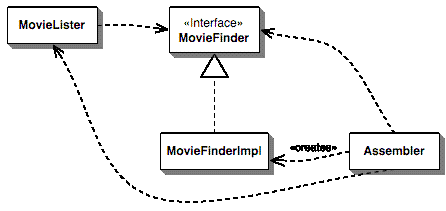
\includegraphics[width=100mm]{images/dependencyinjection.png}
	\caption{Dependency Injection nach Martin Fowler}
	\label{fig:dpendencyinjection}
\end{figure}
Die Funktionsweise kann am einfachsten anhand des Beispiels von Martin Fowler in Abbildung ~\ref{fig:dpendencyinjection} aufgezeigt werden. Die Klasse MovieLister zeigt und filtert Filme, dabei spielt die Quelle woher die Filme kommen keine Rolle. MovieLister benötigt nur eine Liste von Filmen (Abhängigkeit). Die MovieFinderImpl Klasse bietet genau diese Möglichkeit und zeigt dies durch die Implementation des MovieFinder Interfaces an. Der Assembler fügt die Abhängigkeit in den MovieLister ein (Injection).
\\
In dieser Weise können die Filme in einer Excel Datei, in einer Datenbank oder in einer Textdatei gespeichert werden, die Klasse MovieLister kann in jedem Fall verwendet werden.

\subsection{Spring Framework}
Für die Entwicklung von Webapplikationen bietet Spring das integrierte Modul \textit{MVC} an, damit werden die Grundlegenden Funktionalitäten einer Webapplikationen bereits abgedeckt.

\begin{figure}[H]
	\centering
	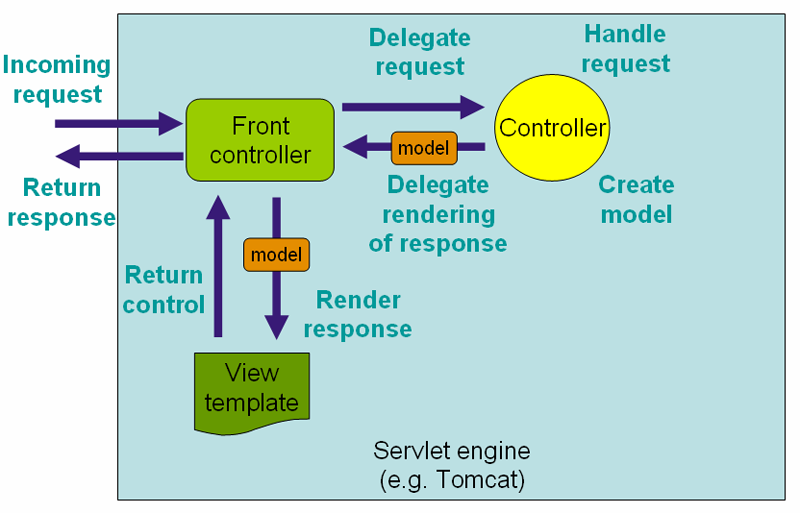
\includegraphics[width=130mm]{images/springmvc.png}
	\caption{Aufbau von Spring MVC \cite{springsourcemvc2011}}
	\label{fig:springmvc}
\end{figure}

Die Anfragen werden durch den Front Controller empfangen und an den passenden Controller der Applikation weitergeleitet. Dieser fügt die angeforderten Daten (Model) hinzu. Das Model wird dann in die View Templates eingefügt und via den Front Controller an den Client zurückgeschickt.
\\
Dieses Abstrakte vorgehen kann durch ein konkretes Beispiel sehr gut dargestellt werden. Eine Anfrage wird durch den Aufruf einer URL im Browser ausgelöst (z.B. http://www.tourlive.ch/rennen). Der Front Controller sucht den Applikations Controller für die Ressource \textit{/rennen}. Bereitet das Model, in diesem Fall alle sichtbaren Rennen, vor und sendet dieses zurück. Der Front Controller sucht den View Resolver übergibt das Model (alle sichtbaren Rennen). Dort wird das Model zur Darstellung gebracht und schlussendlich via den Front Controller an den Browser zurückgesendet. Für jede Ressource gibt es also einen Controller, dabei können aber auch generische Elemente wie z.B. der Rennname in der Ressource verwendet werden (z.B. http://www.tourlive.ch/rennen/tourdesuisse).

\subsubsection{ORM und Datenbank}
Für die Persistierung sämtlicher Daten wird die MySQL ähnliche, quelloffene Datebank MariaDB\footnote{MariaDB, \url{https://mariadb.org/}, aufgerufen am 16.05.2013} verwendet. Dies ist eine Anforderung des Industriepartners cnlab AG.
\\
Die Abbildung des Models auf der Datenbank übernimmt das Java ORM Framework Hibernate\footnote{Hibernate ORM, \url{http://www.hibernate.org/}, aufgerufen am 16.05.2013}, dank unzähliger Datenbanktreiber kann ein beliebiges Datenbanksystem, unter anderem auch MariaDB, verwendet werden.

\subsubsection{Maven}
Für die Verwaltung der externen Java Libraries wird Apache Maven\footnote{Apache Maven, \url{http://maven.apache.org/}, aufgerufen am 16.05.2013} verwendet. Maven lädt die definierten Abhängigkeiten automatisch und kompiliert das Projekt. Weiter generiert Maven die Javadoc\footnote{Javadoc, \url{http://de.wikipedia.org/wiki/Javadoc}, aufgerufen am 16.05.2013} Dokumentation zum Projekt und kann Auswertungen und statische Codeanalysen erzeugen.

\section{Software Design}
